\section{Durchführung}

\subsection{Bau des Roboterarmes}
\schritt{1}{Den Roboterarm vorbereiten}{
Die Pappe schneidet ihr in sechs 30cm lange und 2cm breite Streifen. Davon halbiert ihr zwei, sodass ihr vier 15cm lange Streifen habt. Zwei von diesen kürzt ihr nochmal auf 12cm.\\

\begin{figure}[h]
\centering
\includegraphics[width=5cm]{pappstucke.jpg}
\caption*{Nutzt zum Schneiden entweder eine Schere oder (noch einfacher) Lineal und Cuttermesser. Gut aufpassen und eine schnittfeste Unterlage verwenden!}
\end{figure}

Außerdem benötigt ihr vier Pappteile, die ihr wie auf dem Bild zuschneidet, zirka 12 kleine Pappquadrate und zwei Pappkreise, deren Durchmesser ungefähr mit der Größe der Reifen übereinstimmen sollte. Ein bisschen größer ist ideal.\\

Die Pappstreifen werden jetzt zusammengeklebt. Dafür klebt ihr jeweils zwei gleichlangen Streifen mit Heißkleber zusammen, sodass ihr zwei 30cm, ein 15cm und ein 12cm langes Pappstück habt.\\
Die vier Pappteile klebt ihr übereinander zu einem Klotz. An diesem können später die Stifte mit der Maulklemme befestigt werden.\\
}


\schritt{2}{Den Roboterarm bauen}{
Die Pappteile müssen nun zu einem Arm zusammengebaut werden. Dabei bilden zwei kleine Pappquadrae und ein Zahnstocher ein Gelenk, das die Pappteile miteinander verbindet.

\begin{figure}[h]
\centering
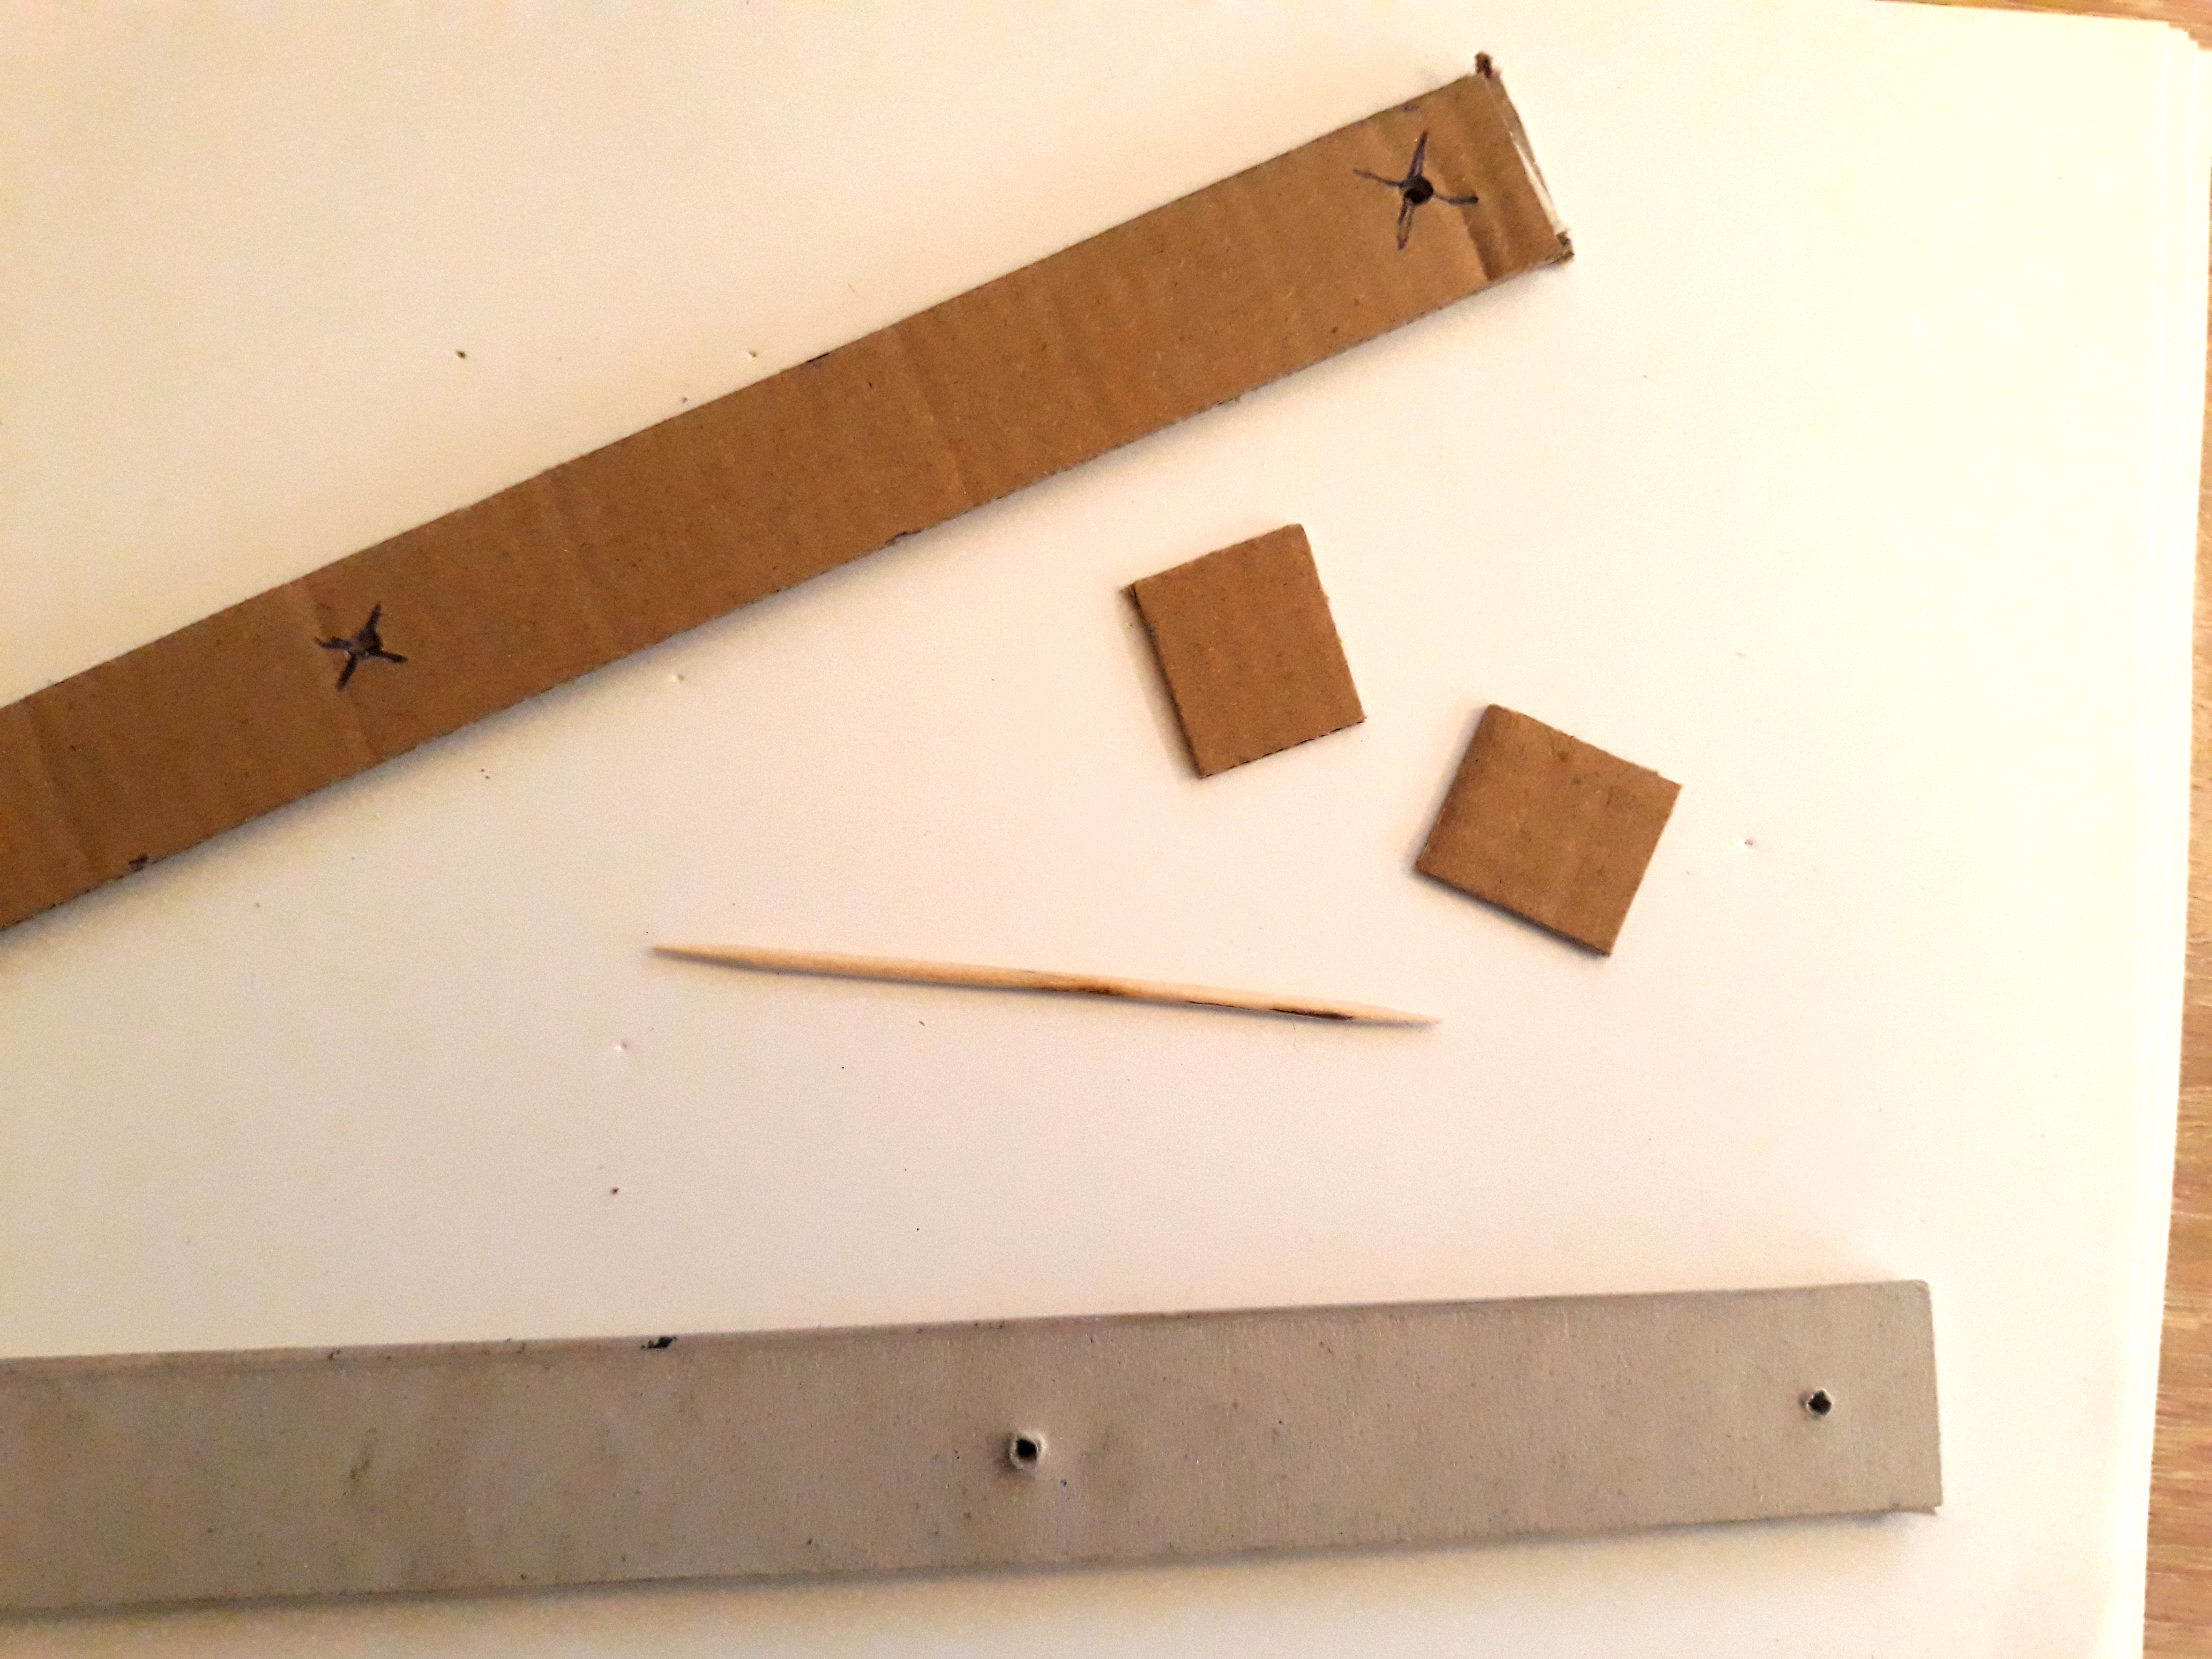
\includegraphics[width=\textwidth]{gelenk.jpg}
\end{figure}


Beim Zusammenstecken der einzelnen Teile orientiert ihr euch am besten an der folgenden Grafik:\\
\begin{figure}[h]
\centering
\includegraphics[width=\textwidth]{arm.jpg}
\end{figure}

Falls ihr nicht weiterwisst, gibt es {https://tuduu.org/projekt/automatischer-malroboter}{hier}\footnote[2]{https://tuduu.org/projekt/automatischer-malroboter} auch nochmal die ausführlichere Beschreibung.\\
Den Pappblock klebt ihr auf die Unterseite des Arms, also nicht die Fläche, auf welcher der zweite Pappstreifen aufliegt.\\

Wenn alles zusammengesteckt und verbunden ist, testet euren Arm vorsichtig. Bewegt sich alles reibungslos?\\
Dann verklebt die Zahnstocher zum Schluss oben und unten mit einem Tropfen Heißkleber, dann hällt alles ein bisschen besser.\\
Die Pappkreise klebt ihr schließlich so auf die Reifen, dass die Pappstreifen oben auf liegen und die Räder sich frei drehen können.\\

Den Stift klebt ihr auf die breite Fläche der Maulklemme. Falls das bei euch (auch) nicht halten sollte, könnt ihr den Stift auch mit der Maulklemme an den Pappklotz klemmen - klappt mindestens genauso gut und hält sicher.\\
Damit ist euer Arm fertig!\\
Weiter geht's mit dem technischen Teil.\\
}



\subsection{Verbindung mit RaspberryPi}

\begin{center}
\includegraphics[width=\textwidth]{rpi_gpio_pinout.png}
\end{center}

\begin{figure}[h]
\centering
\includegraphics[width=5cm]{l298n.png}
\end{figure}

\begin{figure}[h]
\centering
\includegraphics[width=5cm]{treiber_kabel.jpg}
\end{figure}

\begin{figure}[h]
\centering
\includegraphics[width=5cm]{treiber_anschluss_close.jpg}
\end{figure}


Verbindet den Raspberry Pi mit dem Motor sowie den Motor mit dem Treiber mithilfe der folgenden Tabellen.
Für die Verbindungen an den Klemmen des Treibers, öffnet diese zuerst mit einem Schraubendreher, schiebt das Kabel hinein und schraubt sie wieder fest zu. Für die Verbindungen an den Pins verwendet ihr die steckbaren Jumperkabel (sogenannte Female to Female).\\

\schritt{1}{Verbindung der Motoren mit dem Treiber}{}
\begin{table}[h]
  \begin{center}
\begin{tabular}{@{}cc@{}}
\toprule
Motortreiber L298 & 12V Spannungsquelle \\ \midrule
OUT1              & Motor1(+)           \\
OUT2              & Motor1(-)           \\
OUT3              & Motor2(+)           \\
OUT4              & Motor2(-)           \\ \bottomrule
\end{tabular}
\end{center}
\caption{Verbindungen zwischen dem Treiber und den Motoren. Die Polarität der Motoren spielt dabei keine Rolle, ihr müsst euch also keinen Kopf darum machen, ob welches Kabel nach links oder recht muss.}
\end{table}


\schritt{2}{Verbindung des Treibers mit dem Raspberry Pi}{}

\begin{table}[h]
 \begin{center}
\begin{tabular}{@{}cc@{}}
\toprule
Raspberry Pi GPIO                                                & Motortreiber L298                                                                                                                               \\ \midrule
GPIO 20                                                          & IN1                                                                                                                                             \\
GPIO 16                                                          & IN2                                                                                                                                             \\
GPIO 19                                                          & IN3                                                                                                                                             \\
GPIO 4                                                           & IN4                                                                                                                                             \\
GPIO 12                                                          & ENA                                                                                                                                             \\
GPIO 13                                                          & ENB                                                                                                                                             \\
\begin{tabular}[c]{@{}c@{}}Masse (GND)\\ z.B. Pin 6\end{tabular} & \begin{tabular}[c]{@{}c@{}}Masse (GND) - Klemme\\ die selbe Klemme, an die auch (-)\\ der Versorgungsspannung angeschlossen\\ wird\end{tabular} \\ \bottomrule
\end{tabular}
\end{center}
\caption{Verbindungen zwischen dem Raspberry Pi und dem Motortreiber. Die Bezeichnungen des Treibers findet ihr auf der Boardober- oder -unterseite}
\end{table}

Achtet besonders auf die letzte Verbindung in der Tabelle! Am besten verbindet ihr hier mit einem Male-Female Jumperkabel, wie ihr es im Bild oben sehen könnt.\\

\schritt{3}{Verbindung der Versorgungsspannung an den Treiber}{}
Für diese Verbindung eignet sich ein Adapter, der den Stecker des 12V Netzteiles auf zwei einfache Kabel führt, um diese an die Klemmen des Treibers anzuschließen.

% Please add the following required packages to your document preamble:
% \usepackage{booktabs}
\begin{table}[h]
  \begin{center}
\begin{tabular}{@{}cc@{}}
\toprule
Motortreiber L298 & 12V Spannungsquelle          \\ \midrule
+12V              & +12V (i.d.R. rotes Kabel)    \\
GND               & GND (i.d.R. schwarzes Kabel) \\ \bottomrule
\end{tabular}
\end{center}
\caption{Verbindungen zwischen Treiber und Netzteil}
\end{table}

\begin{figure}[h]
\centering
\includegraphics[width=5cm]{netzteil_close.jpg}
\end{figure}


\subsection{Programmierung}
\subsection{Beispielprogramm kurs.py}


\begin{lstlisting}

# setz Geschwindigkeit des ersten Motors auf 20%, dreht links
motorA_links(20)

input("Enter zum fortfahren")

# setz Geschwindigkeit des ersten Motors auf 12%, dreht rechts
motorB_rechts(12)

motorA_aus()
motorB_aus()

\end{lstlisting}

Je nach Python-Kenntnissen kann das Programm noch um weitere Logikblöcke ergänzt werden, zum Beispiel Eingabeabfragen für die Drehgeschwindigkeit der Motoren oder ein ganzes Menü zur Steuerung des Roboters.\\
Das Programm schreibt ihr am besten in der Datei kurs.py, und öffnet und führt es dann in Thonny aus.\\
\hinweis Bei 12Volt und einer Stromversorgung über ein Netzteil sind 10\% Drehgeschwindigkeit der Motoren okay. 50\% sollten aber keinesfalls überschritten werden, die Motoren drehen dann einfach zu stark und zu schnell und könnten den Roboter damit in seine Einzelteile zerlegen. Probiert am besten ein bisschen herum, bevor ihr den Arm mit den Motoren verbindet.\\
